% ______________________________________________________________________________
%
% DVG001 -- Introduktion till Linux och små nätverk
%                              Inlämningsuppgift #4
% ~~~~~~~~~~~~~~~~~~~~~~~~~~~~~~~~~~~~~~~~~~~~~~~~~
% Author:   Jonas Sjöberg
%           tel12jsg@student.hig.se
%
% Date:     2016-04-06 -- 2016-04-11
%
% License:  Creative Commons Attribution 4.0 International (CC BY 4.0)
%           <http://creativecommons.org/licenses/by/4.0/legalcode>
%           See LICENSE.md for additional licensing information.
% ______________________________________________________________________________


\section{Del ett}
% TODO: introduktion till del 1


% ______________________________________________________________________________
\subsection{\texttt{IP}-nummer}
\subsubsection{Uppgiftsbeskrivning}
Här är uppgiften att ta reda på vilken \texttt{IP}-adress som maskinen har samt
hur den fått sin adress genom att använda kommandot \texttt{ip} och titta i
loggar, exempelvis \texttt{/var/log/messages}.


\subsubsection{Lösning}
För att ta reda på datorns \texttt{IP}-adress körs kommandot i
Programlistning~\ref{listing:sh_1-ip}.

\begin{listing}[H]
  \shellcode{include/sh_1-ip}
  \caption{Kommando för att ta reda på datorns \texttt{IP}-adress.}
  \label{listing:sh_1-ip}
\end{listing}

Resultatet visar att datorns \texttt{IP}-adress är \texttt{192.168.1.112}
med nätmasken \texttt{24}.

Ett shell-skript används för att söka igenom loggar efter den aktuella
\texttt{IP}-adressen. Programmet letar efter filer i sökvägen \texttt{/var/log}
och undersöker filernas innehåll genom att läsa ''magic header bytes'' som
avgör vilken typ av fil det är. Om en hittad fil är en vanlig textfil söks dess
innehåll efter datorns aktuella \texttt{IP}-adress som extraherats tidigare.

Programmet visas i Programlistning~\ref{listing:sh_1-grep-logs.sh} och
resultatet av en körning visas i
Figur~\ref{fig:sh_1-grep-logs.sh_output}

\begin{listing}[H]
  \shellcode{include/sh_1-grep-logs.sh}
  \caption{Kommando för att söka igenom loggar i sökvägen \texttt{/var/log}
           efter omnämnanden av datorns aktuella \texttt{IP}-adress.}
  \label{listing:sh_1-grep-logs.sh}
\end{listing}

\begin{figure}[htp]
  \centering
  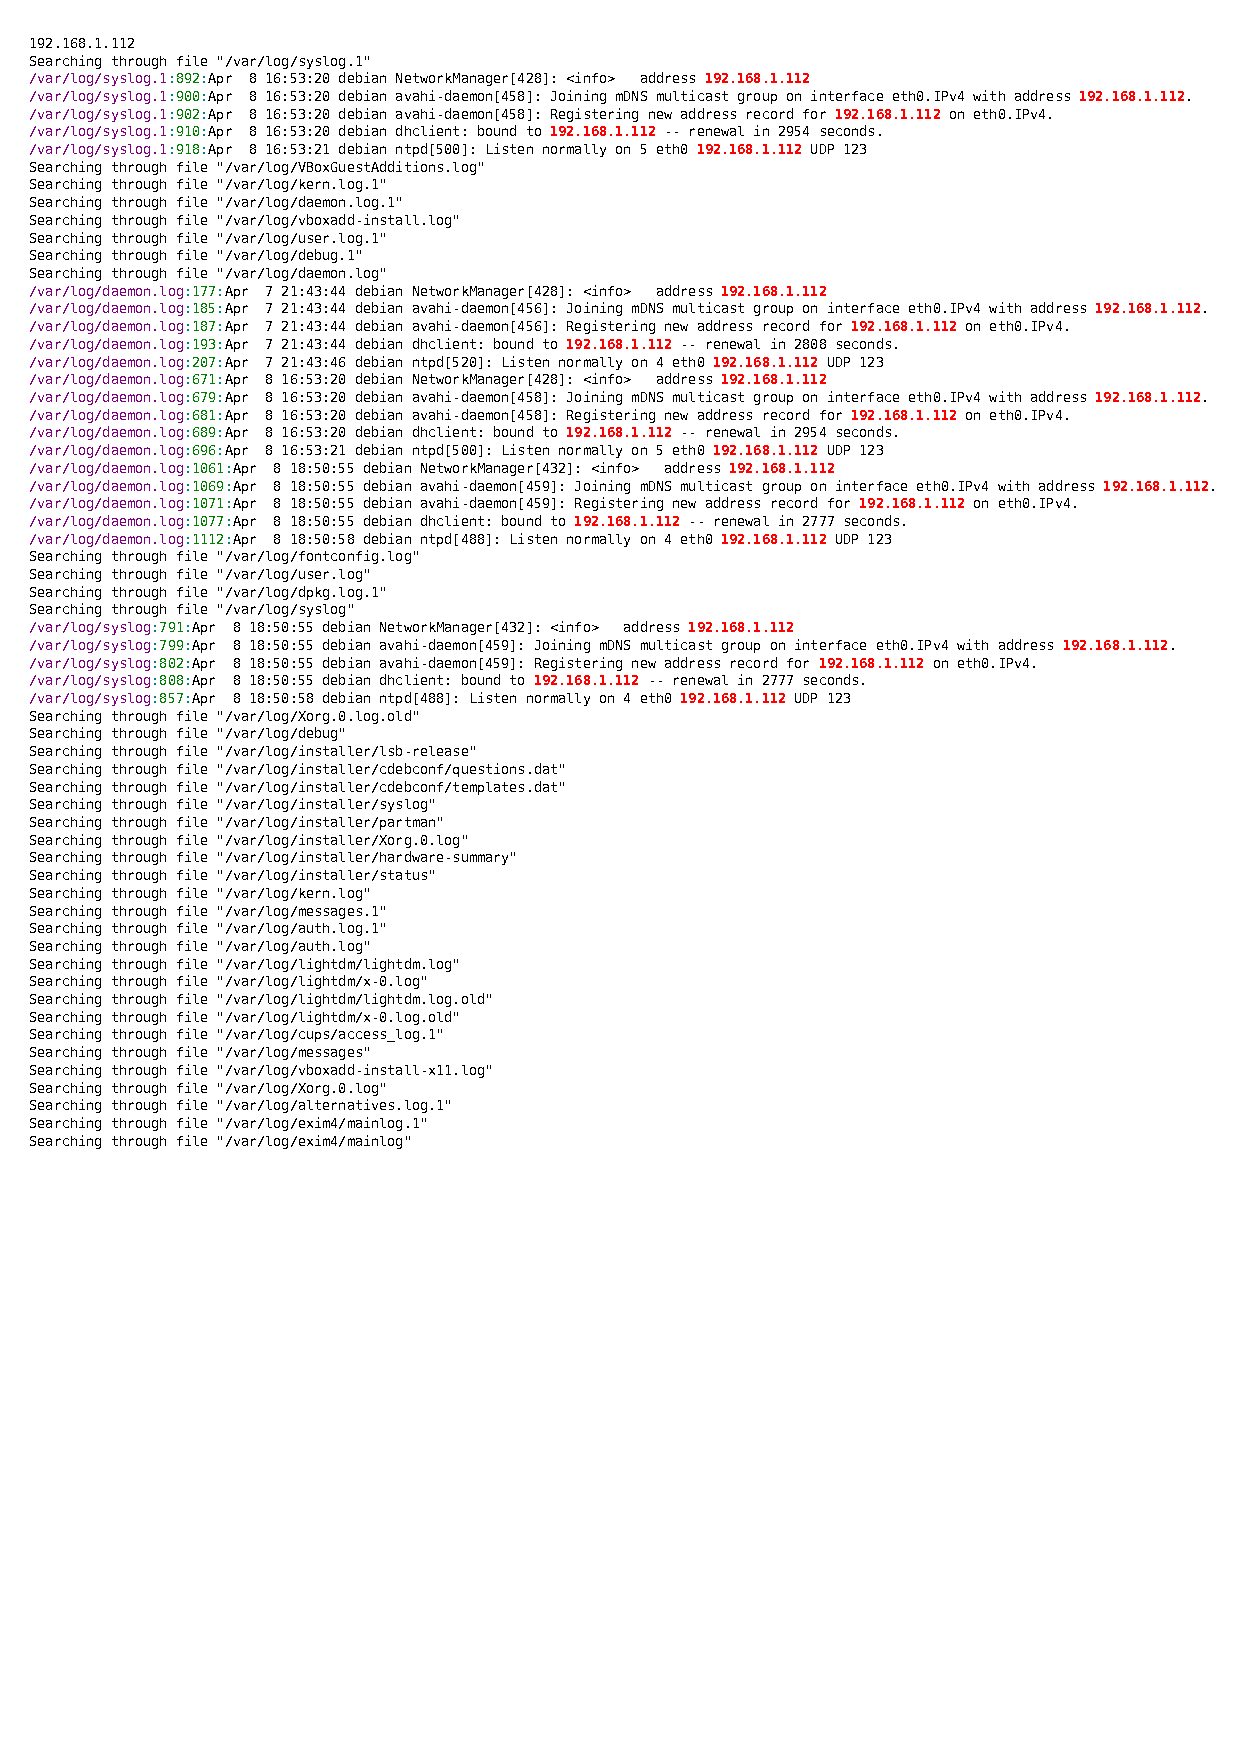
\includegraphics[scale=0.85]{include/sh_1-grep-logs-sh_output.pdf}
  \caption{Körning av programmet i Programlistning~\ref{listing:sh_1-grep-logs.sh}.}
  \label{fig:sh_1-grep-logs.sh_output}
\end{figure}

Bland resultaten finns omnämnanden av \texttt{mDNS} som rör \texttt{DHCP}.
Instruktionerna nämner också att den grafiska miljön har verktyg för att
konfigurera nätverksinställningar, en skärmdump på detta visas i
Figur~\ref{fig:scr_1-network_A} och Figur~\ref{fig:scr_1-network_B} .

\begin{figure}[htp]
  \centering
  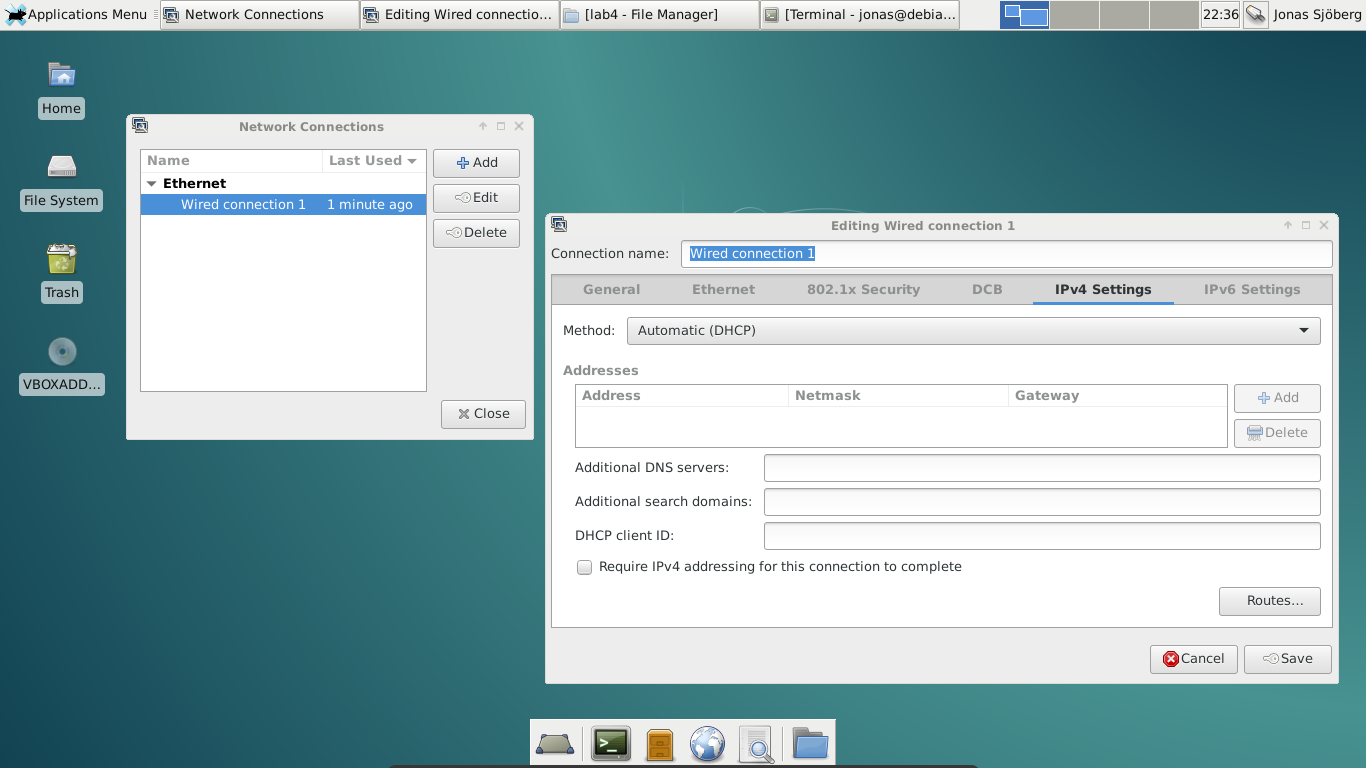
\includegraphics[scale=0.35]{include/scr_1-network_A.png}
  \caption{Nätverksinställningar i det grafiska gränssnittet.}
  \label{fig:scr_1-network_A}
\end{figure}

\begin{figure}[htp]
  \centering
  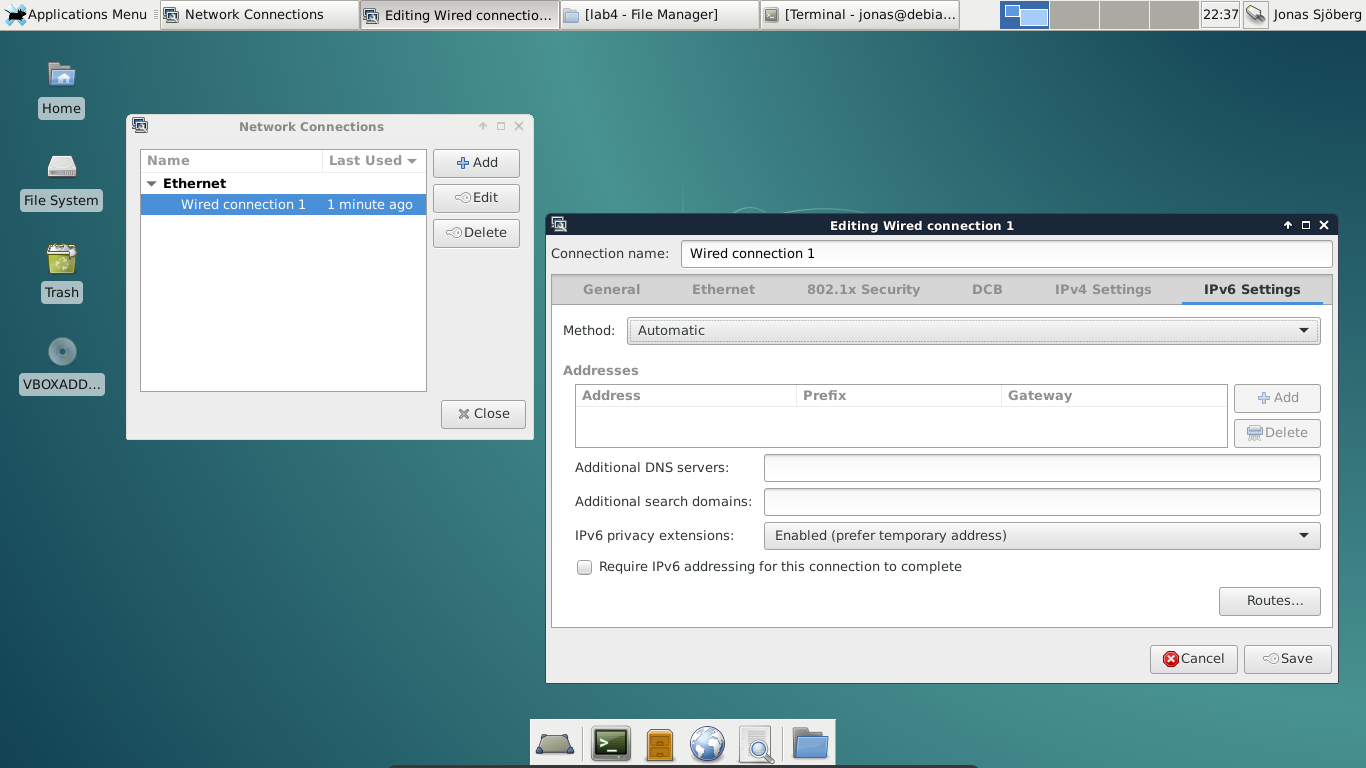
\includegraphics[scale=0.35]{include/scr_1-network_B.png}
  \caption{Nätverksinställningar i det grafiska gränssnittet.}
  \label{fig:scr_1-network_B}
\end{figure}


% ______________________________________________________________________________
\subsection{Nät- och Nodnummer}
\subsubsection{Uppgiftsbeskrivning}
Uppgiften är här att ange vilken nätadress man har genom att använda
\texttt{CIDR} och dessutom ange nätmasken.


\subsubsection{Lösning}
För detaljerad information om datorns \texttt{IP}-adress körs kommandot i
Programlistning~\ref{listing:sh_1-ipcalc}. Resultatet av körningen visas i
Figur~\ref{fig:sh_1-ipcalc_output}

\begin{listing}[H]
  \shellcode{include/sh_1-ipcalc}
  \caption{Kommando för att visa detaljerad information om en
           \texttt{IP}-adress.}
  \label{listing:sh_1-ipcalc}
\end{listing}

\begin{figure}[htp]
  \centering
  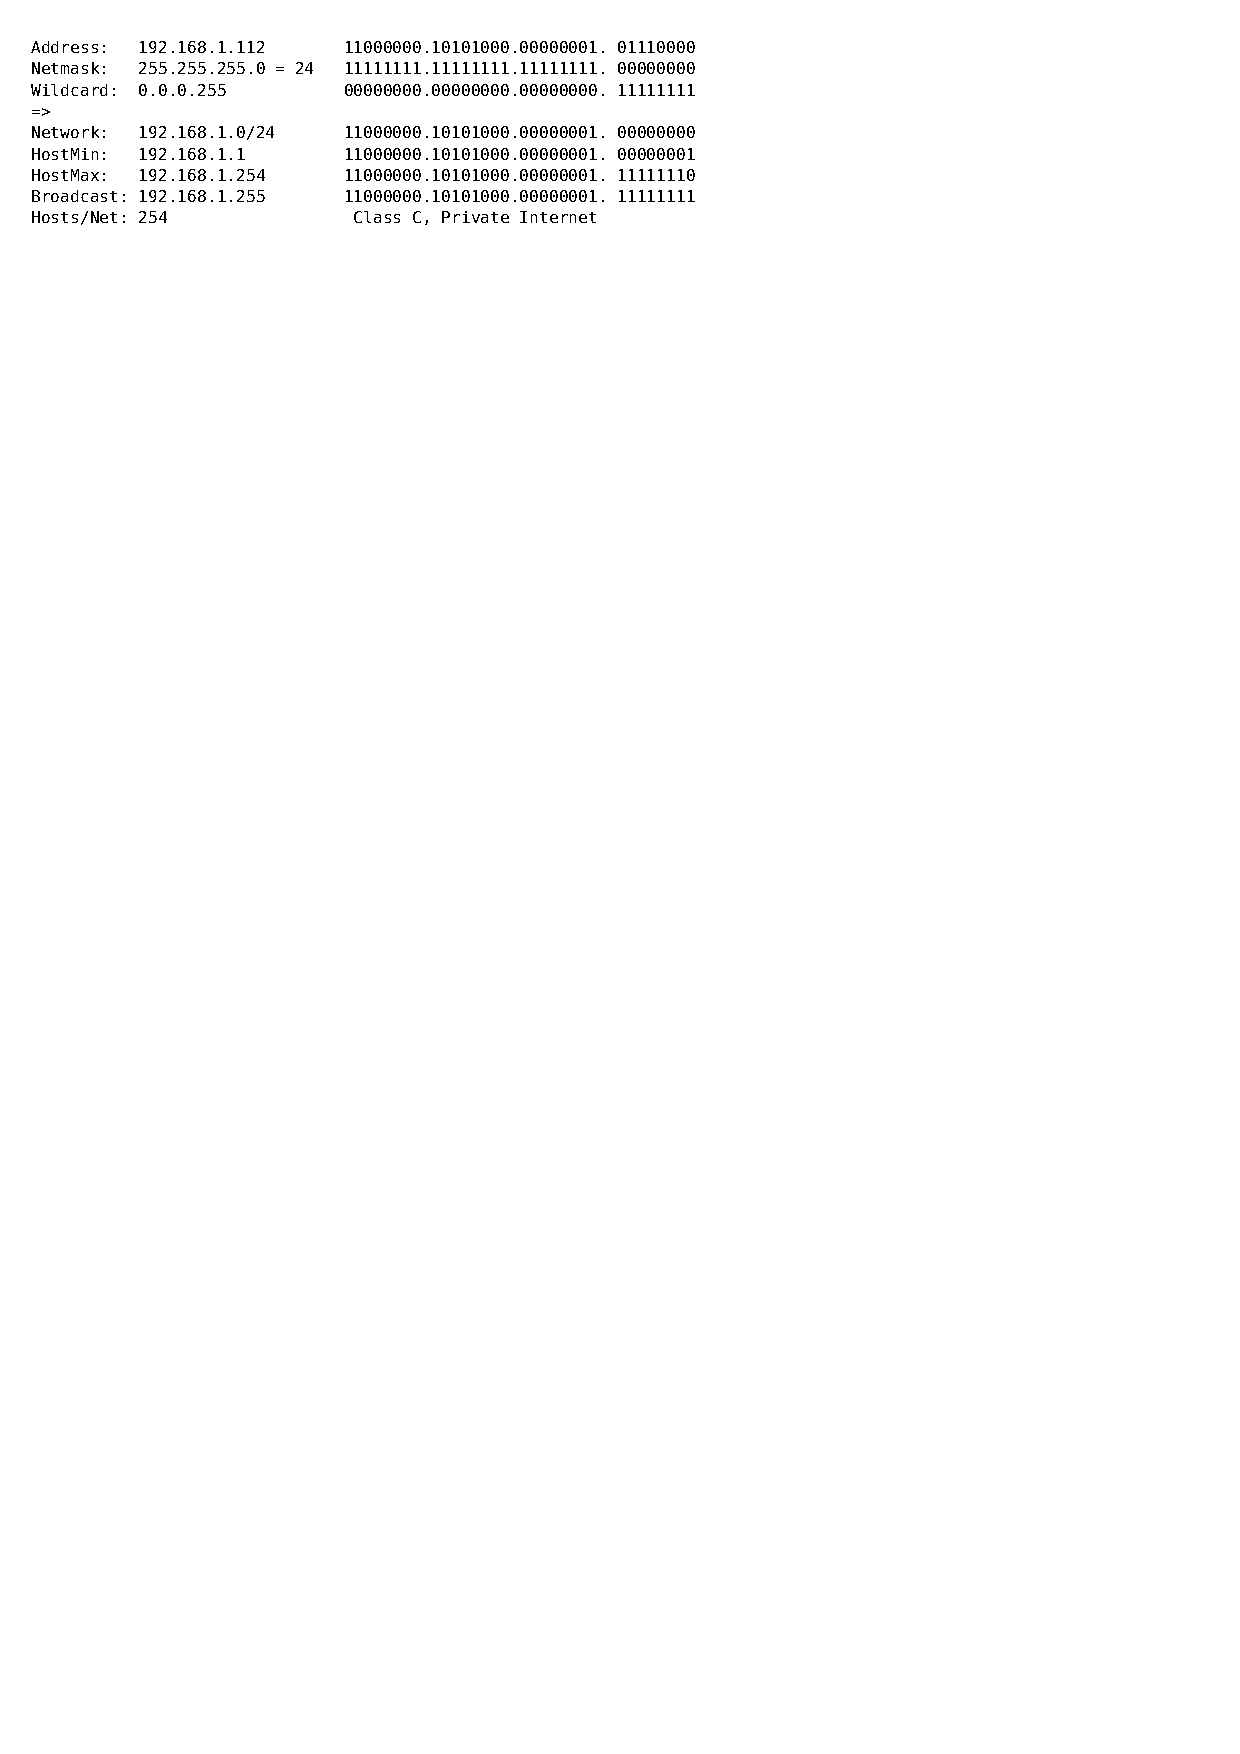
\includegraphics[scale=0.85]{include/sh_1-ipcalc_output.pdf}
  \caption{Körning av programmet i Programlistning~\ref{listing:sh_1-ipcalc}.}
  \label{fig:sh_1-ipcalc_output}
\end{figure}



% ______________________________________________________________________________
\subsection{Routeradresser}
\subsubsection{Uppgiftsbeskrivning}
Uppgiften är att lista de routrar som maskinen känner till och dessutom ange
vilken som är standardroutern.

\subsubsection{Lösning}
För att få en lista på routrar som datorn känner till används kommandot \texttt{ip route list}.
Körning med resultat visas i Programlistning~\ref{listing:sh_1-ip-route-list}.

\begin{listing}[H]
  \shellcode{include/sh_1-ip-route-list}
  \caption{Körning av kommando för att lista information om routers på nätverk.}
  \label{listing:sh_1-ip-route-list}
\end{listing}

Resultatet visar att standard-routern har \texttt{IP}-adress \texttt{192.168.1.1}.

Lite mer detaljerad men i stort sett samma information kan fås med \texttt{ip
neighbor} som i Programlistning~\ref{listing:sh_1-ip-neighbor}. 

\begin{listing}[H]
  \shellcode{include/sh_1-ip-neighbor}
  \caption{Körning av kommando för att lista information maskiner i samma nät.}
  \label{listing:sh_1-ip-neighbor}
\end{listing}

Anmärkningsvärt är att datorn rapporterar att den enhet som används är av typen
\texttt{eth0}.  Men eftersom att datorn körs som en virtuell maskin på en
laptop som ansluter till nätverket genom en trådlös WIFI-anslutning så är det
uppenbarligen inte sant.  Den trådbundna anslutningen är virtuell och skapas av
\texttt{VirtualBox}.

% ______________________________________________________________________________
\subsectionM{\texttt{MAC}-adresser}
\subsubsection{Uppgiftsbeskrivning}
Här är uppgiften att lista \texttt{MAC}- och \texttt{IP}-adresser för alla
maskiner i nätverket.

\subsubsection{Lösning}

För mer avancerade möjligheter används programmet \texttt{nmap}, som enkelt kan
installeras från paketarkiven med t.ex. \texttt{apt}.  Programmet \texttt{nmap}
är väldigt kraftfullt och har många användningsområden.  I det här fallet körs
\texttt{nmap -sn -v 192.168.1.1/24}.  Flaggan \texttt{-sn} innebär att
\texttt{nmap} kör en enklare typ av skanning, ''no port scan'', ''ping scan''
eller ''ping sweep''.

Följande beskrivning är hämtad ur manualsidan för \texttt{nmap(1)}
\cite{manpage:nmap}:

\begin{quotation}
When  the  server  is  unreachable, send a burst of eight packets
instead of the usual one.  The packet spacing is normally 2 s; however, the
spacing between the first and second packets can be changed with the calldelay
command to allow additional time for a modem or ISDN call to  complete.   This
option is valid with only the server command and is a recommended option with
this command.
\end{quotation}

\begin{quotation}
Systems administrators often find this option valuable as well. It can easily
be used to count available machines on a network or monitor server
availability. This is often called a ping sweep, and is more reliable than
pinging the broadcast address because many hosts do not reply to broadcast
queries.

The default host discovery done with -sn consists of an ICMP echo request, TCP
SYN to port 443, TCP ACK to port 80, and an ICMP timestamp request by default.
When executed by an unprivileged user, only SYN packets are sent (using a
connect call) to ports 80 and 443 on the target. When a privileged user tries
to scan targets on a local ethernet network, ARP requests are used unless
--send-ip was specified. 
\end{quotation}

Vidare ökar flaggar \texttt{-v} mängden text (''verbose mode'') och 
\texttt{IP}-adresserna 


Även om \texttt{nmap} i det här fallet gott kan anses vara ''overkill'' så är
det användbart i många scenarion och därför bra att känna till.

Körningen visas i Programlistning~\ref{listing:sh_1-nmap-sn}.  Resultatet är
delvis ''censurerat'' av säkerhetsskäl.

\begin{listing}[H]
  \shellcode{include/sh_1-nmap-sn}
  \caption{Körning av portskannern \texttt{nmap} för att lista datorer på
           nätverket. Resultatet är ''censurerat'' av säkerhetsskäl.}
  \label{listing:sh_1-nmap-sn}
\end{listing}


Resultatet redovisas även i Tabell~\ref{table:network}.

\begin{table}[]
  \centering
  \caption{Lista över \texttt{MAC}- och \texttt{IP}-adresser för maskiner på
           nätverket.}
  \label{table:network}
  \begin{tabular}{@{}llll@{}}
    \toprule
    \texttt{IP}-adress     & \texttt{MAC}-address       & Enhetens tillverkare          \\ \midrule
    \texttt{192.168.1.1}   & \texttt{04:EC:08:A7:8B:A0} & Tp-link Technologies CO.      \\
    \texttt{192.168.1.101} & \texttt{08:9E:0C:A4:50:30} & Apple                         \\
    \texttt{192.168.1.106} & \texttt{0C:3A:01:9C:23:F0} & Samsung Electro Mechanics CO. \\
    \texttt{192.168.1.107} & \texttt{00:26:02:5A:76:40} & Gemtek Technology Co.         \\
    \texttt{192.168.1.108} & \texttt{04:81:09:CD:C9:40} & Canon                         \\
    \texttt{192.168.1.110} & \texttt{04:11:0B:37:FC:90} & Hewlett Packard               \\ \bottomrule
  \end{tabular}
\end{table}



